\documentclass[11pt]{beamer}
\usepackage{tikz}
\usetikzlibrary{decorations.pathreplacing}
\usepackage{verbatim}
\usepackage{tkz-berge}
\usepackage{algpseudocode}
\usepackage{tikz}
\usepackage[labelformat=empty]{caption}
\usetikzlibrary{calc,fit}
\usetheme{Frankfurt}

\title[Drug-Target Interaction Prediction by Integrating Chemical, Genomic, Functional and Pharmacological Data] % (optional, only for long titles)
{Drug-Target Interaction Prediction by Integrating Chemical, Genomic, Functional and Pharmacological Data}
\subtitle{Fan Yang, Jinbo Xu, Jianyang Zeng\\2014, Pacific Symposium on Biocomputing}
\author[] % (optional, for multiple authors)
{Marten Heidemeyer}
\date[\today] % (optional)
{Presentation for Directed Reading Class, Summer 2015}
\subject{Probabilistic Graphical Models}

\begin{document}
\setbeamertemplate{caption}{\raggedright\insertcaption\par}
\frame{\titlepage}
\begin{frame}
\frametitle{Outline}
\tableofcontents[]
\end{frame}

\section{Motivation}
\begin{frame}
\frametitle{Motivation}
Knowledge of Drug-Target interaction is important for:
\begin{itemize}
\item drug development
\item predicting drug side effects
\item identification of new targets for known drugs
\end{itemize}
Wet lab experiments for Drug-Target interaction are expensive
\end{frame}
\begin{frame}
\frametitle{Available Resources}
\begin{itemize}
\item binary/real-value interaction data
\begin{itemize}
\item KEGG, BRENDA, SuperTarget, DrugBank, BindingDB
\item KEGG: 875 Drugs, 249 Proteins, 2596 observations
\item BindingDB: 106527 Ligands, 2133 Proteins, 193603 observations
\end{itemize}
\item KEGG: chemical structure of drugs
\item SIDER: drug side effect database
\item KEGG: protein sequence of targets
\item GO: functional annotation of targets
\pause
\item Goal: integrate genomic, chemical, functional and pharmacological data to predict missing interactions
\end{itemize}
\end{frame}

\section{Method}
\begin{frame}
\frametitle{Conditional Random Field structure}
We have given:
\begin{center}
drugs: $d_i$, $1\leq i \leq n_d$\\
targets: $t_j$, $1\leq j \leq n_t$\\
\end{center}
For each drug $d_i$, construct CRF over:
\begin{center}
$G=(V_t, E_t)$, where $V_t$ set of all targets\\
$E_t:$ connect each target to its $k$ nearest neighbors \\

\begin{center}
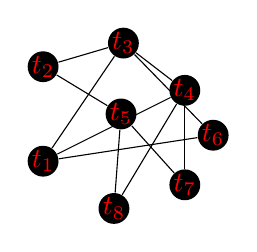
\begin{tikzpicture}[scale=0.3]
\tikzstyle{vertex}=[circle,fill=black,minimum size=9pt,inner sep=0pt]
\foreach \name/\point in {
	1/{-1,-1},
	2/{-1,3},
	3/{2.4,4},
	4/{5,2.0},
	5/{2.3,1},
	6/{6.2,0.1},
	7/{5,-2},
	8/{2,-3}}
 	\node[vertex] (\name) at (\point) {\color{red}$t_{\name}$};
 	\draw (2) -- (3) node[draw=none,fill=none,midway,above,font=\tiny] {};
 	\draw (2) -- (5) node[draw=none,fill=none,midway,below,near start,font=\tiny] {};
 	\draw (1) -- (4) node[draw=none,fill=none,midway,below,font=\tiny, near end] {};
 	\draw (1) -- (3) node[draw=none,fill=none,left,font=\tiny,near start] {};
 	\draw (6) -- (3) node[draw=none,fill=none,left,font=\tiny,near start] {};
 	\draw (4) -- (3) node[draw=none,fill=none,left,font=\tiny,near start] {};
 	\draw (4) -- (7) node[draw=none,fill=none,left,font=\tiny,near start] {};
 	\draw (4) -- (8) node[draw=none,fill=none,left,font=\tiny,near start] {};
 	\draw (5) -- (7) node[draw=none,fill=none,left,font=\tiny,near start] {};
 	\draw (5) -- (8) node[draw=none,fill=none,left,font=\tiny,near start] {};
 	\draw (6) -- (1) node[draw=none,fill=none,left,font=\tiny,near start] {};
\end{tikzpicture}
\end{center}

\end{center}

\end{frame}

\begin{frame}
\frametitle{Conditional Random Field structure}
We have given:
\begin{center}
drugs: $d_i$, $1\leq i \leq n_d$\\
targets: $t_j$, $1\leq j \leq n_t$\\
\end{center}
For each drug $d_i$, construct CRF over:
\begin{center}
$G=(V_t, E_t)$, where $V_t$ set of all targets\\
$E_t:$ connect each target to its $k$ nearest neighbors 
\end{center}
Do the same for each target $t_i$, where nodes are the drugs.

\end{frame}

\begin{frame}
\frametitle{formal definition of CRF}
Let $Y=(y_1, y_2, \dots, y_{n_t})$ denote the prediction of target $t_j$.\\
Let $X$ denote known DTIs and similarity scores.\\
Define the joint probability density function of $Y$ given $X$:
\begin{center}
$p(Y|X)=\frac{1}{Z(X)}e^{-E(Y|X)}$\\
\pause
$Z(X)=\sum_Y e^{-E(Y|X)}$
\end{center}
\pause
Definition of CRF from book:
\begin{center}
$P(Y|X)=\frac{1}{Z(X)}\tilde{P}(Y,X)$\\
$\tilde{P}(Y,X)=\prod\limits_i^m\phi_i(D_i)$\\
$Z(X)=\sum_Y \tilde{P}(Y,X)$
\end{center}
\end{frame}



\begin{frame}
\frametitle{formal definition of CRF 2}
For joint configuration $Y$ given $X$, define energy:
\begin{center}
$E(Y|X)=\sum\limits_i a_i f(y_i|X) + \sum\limits_{i,j} b_{ij} g(y_i, y_j~|X)$
\end{center}
where $f$ and $g$ are penalty functions:
\begin{center}
$f(y_i|X) = -(y_i -H_{x_i}(y_i))^2$, where\\
$H_{x_i}(y_i)$ average number of observed interactions for $t_i$\\
\end{center}
\pause
and
\begin{center}
$g(y_i,y_j|X) = -H_{x_i,x_j}(y_i-y_j)^2$, where \\
$H_{x_i, x_j}(y_i-y_j) = 0$, if no edge between $t_i$ and $t_j$
\end{center}
we learn $a_i$ and $b_{ij}$.
\end{frame}

\begin{frame}
\frametitle{Example: Target-Based CRF}
\begin{center}
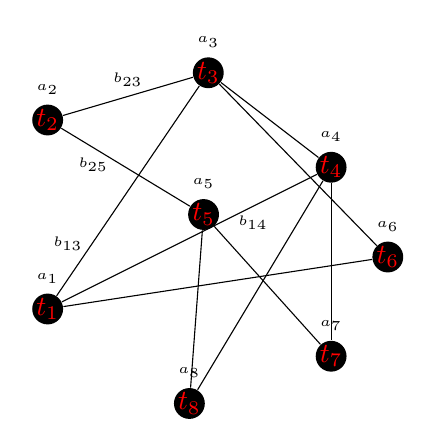
\begin{tikzpicture}[scale=0.6]
\tikzstyle{vertex}=[circle,fill=black,minimum size=9pt,inner sep=0pt,label={[font=\tiny] $a_{\name}$}]
\foreach \name/\point in {
	1/{-1,-1},
	2/{-1,3},
	3/{2.4,4},
	4/{5,2.0},
	5/{2.3,1},
	6/{6.2,0.1},
	7/{5,-2},
	8/{2,-3}}
 	\node[vertex] (\name) at (\point) {\color{red}$t_{\name}$};
 	\draw (2) -- (3) node[draw=none,fill=none,midway,above,font=\tiny] {$b_{23}$};
 	\draw (2) -- (5) node[draw=none,fill=none,midway,below,near start,font=\tiny] {$b_{25}$};
 	\draw (1) -- (4) node[draw=none,fill=none,midway,below,font=\tiny, near end] {$b_{14}$};
 	\draw (1) -- (3) node[draw=none,fill=none,left,font=\tiny,near start] {$b_{13}$};
 	\draw (6) -- (3) node[draw=none,fill=none,left,font=\tiny,near start] {};
 	\draw (4) -- (3) node[draw=none,fill=none,left,font=\tiny,near start] {};
 	\draw (4) -- (7) node[draw=none,fill=none,left,font=\tiny,near start] {};
 	\draw (4) -- (8) node[draw=none,fill=none,left,font=\tiny,near start] {};
 	\draw (5) -- (7) node[draw=none,fill=none,left,font=\tiny,near start] {};
 	\draw (5) -- (8) node[draw=none,fill=none,left,font=\tiny,near start] {};
 	\draw (6) -- (1) node[draw=none,fill=none,left,font=\tiny,near start] {};
\end{tikzpicture}
\end{center}
\end{frame}

\begin{frame}
\frametitle{CRF: Parameter Training}
learn  $a_i$ and $b_{ij}$ by maximizing the conditional log-likelihood of training data.\\
\pause
conditional probability was defined as:
\begin{center}
$p(Y|X)=\frac{1}{Z(X)}e^{-E(Y|X)}$\\
\pause
$\Rightarrow p_\theta(Y|X) = \frac{1}{Z_{\theta}(X)}e^{\theta h}$
\end{center}
$\Rightarrow$ log-likelihood:
\begin{center}
$L_{\theta}=\sum\limits_{i=1}^{n_t}log(p(y_i|X))$\pause $\bigg \vert \theta = (e^{\theta_1^{'}},\dots,e^{\theta_{n_t}^{'}})$\\
\end{center}
$\Rightarrow$ derivative of log-likelihood:
\begin{center}
$\frac{\delta L_{\theta}}{\delta \theta^{'}}=\theta\sum\limits_{i=1}^{n_t}h(y_i|X)-E_\theta(h(Y|X))$
\end{center}
\begin{itemize}
\item use \textit{stochastic gradient ascent} to find maximizing $\theta$\\
\item use \textit{contrastive divergence} to deal with $E_\theta(h(Y|X))$
\end{itemize}
\end{frame}

\begin{frame}
\frametitle{Example: Target-Based CRF}
\begin{center}
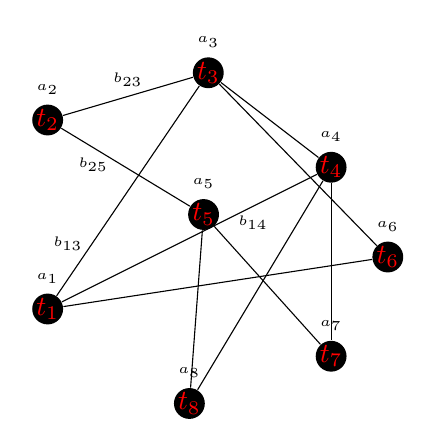
\begin{tikzpicture}[scale=0.6]
\tikzstyle{vertex}=[circle,fill=black,minimum size=9pt,inner sep=0pt,label={[font=\tiny] $a_{\name}$}]
\foreach \name/\point in {
	1/{-1,-1},
	2/{-1,3},
	3/{2.4,4},
	4/{5,2.0},
	5/{2.3,1},
	6/{6.2,0.1},
	7/{5,-2},
	8/{2,-3}}
 	\node[vertex] (\name) at (\point) {\color{red}$t_{\name}$};
 	\draw (2) -- (3) node[draw=none,fill=none,midway,above,font=\tiny] {$b_{23}$};
 	\draw (2) -- (5) node[draw=none,fill=none,midway,below,near start,font=\tiny] {$b_{25}$};
 	\draw (1) -- (4) node[draw=none,fill=none,midway,below,font=\tiny, near end] {$b_{14}$};
 	\draw (1) -- (3) node[draw=none,fill=none,left,font=\tiny,near start] {$b_{13}$};
 	\draw (6) -- (3) node[draw=none,fill=none,left,font=\tiny,near start] {};
 	\draw (4) -- (3) node[draw=none,fill=none,left,font=\tiny,near start] {};
 	\draw (4) -- (7) node[draw=none,fill=none,left,font=\tiny,near start] {};
 	\draw (4) -- (8) node[draw=none,fill=none,left,font=\tiny,near start] {};
 	\draw (5) -- (7) node[draw=none,fill=none,left,font=\tiny,near start] {};
 	\draw (5) -- (8) node[draw=none,fill=none,left,font=\tiny,near start] {};
 	\draw (6) -- (1) node[draw=none,fill=none,left,font=\tiny,near start] {};
\end{tikzpicture}
\end{center}
\pause
\begin{itemize}
\item all Target-Based CRFs share the same $a_i$ and $b_{ij}$.
\pause
\item exact same procedure for construction of Drug-Based CRFs.
\end{itemize}
\end{frame}

\begin{frame}
\frametitle{Predicting New Drug-Target Interactions}
prediction for target $t_k$:\\
\begin{itemize}
\item previously we learned $P(Y|X)$
\item compute conditional probability distribution $p(y_k|y_{-k},X)$
\begin{itemize}
\item $y_{-k}$: all other targets except $t_k$, set this value to $1$ if target is known to interact with query drug, and $0$ otherwise
\item $p(y_k|y_{-k},X)=\frac{p(Y|X)}{p(y_{-k}|X)}$
\end{itemize}
\item prediction score: conditional expectation of $y_k$
\item reminder:
\begin{center}
$E(Y|X)=\sum\limits_i a_i f(y_i|X) + \sum\limits_{i,j} b_{ij} g(y_i, y_j~|X)$
\end{center}
\end{itemize}
\end{frame}

\begin{frame}
\frametitle{Construction of CRF}
Different approaches to define edges:
\begin{itemize}
\item target-based CRF: sequence similarity measure (Genomic approach)
\item target-based CRF: functional similarity measure (Functional approach)
\item target-based CRF: OR of Genomic and Functional measure (Integrated Genomic-Functional approach)
\pause
\item drug-based CRF: chemical similarity measure (Chemical approach)
\item drug-based CRF: side effect similarity measure (Pharmacological approach)
\item drug-based CRF: OR of Chemical and Pharmacological measure (Integrated Chemical-Pharmacological approach)
\end{itemize}
\end{frame}

\begin{frame}
\frametitle{Full Integration approach}
For a given drug-target pair:
\begin{itemize}
\item let $S_d$ denote prediction score using the drug-based CRF 
\item let $S_t$ denote prediction score using the target-based CRF
\end{itemize}
Compute score for this query drug-target pair as
\begin{center}
$S=\alpha S_d + (1-\alpha) S_t$
\end{center}
\end{frame}

\section{Results}
\begin{frame}
\frametitle{Testdata and similarity metrics}
\begin{itemize}
\item experimentally-verified drug-target interactions from $KEGG$ database.
\item 875 drugs, 249 proteins, 2596 tested interactions $\Rightarrow$ 0.4\% 
\item graph kernel approach to compute chemical similarities between drugs.
\item local alignment kernel approach to compute sequence similarities between targets.
\item $FunSimMat$ to compute functional similarities between targets.
\item pharmacological information from $SIDER$ database.
\end{itemize}
\end{frame}

\begin{frame}
\frametitle{Performance Evaluation}
\begin{center}
\begin{figure}
\includegraphics[scale=0.4]{table1} 
\caption{Table 1: Prediction results using 10-fold cross validation}
\end{figure}
\end{center}
\end{frame}

\begin{frame}
\frametitle{Comparison with existing approaches}
\begin{itemize}
\item $KEGG$ dataset, where all drugs have records in drug side-effects databases $SIDER$, $JAPIC$ and $AERS$
\item 359 drugs, 226 targets, 1188 drug-target interactions $\Rightarrow$ 1.4\%
\end{itemize}

\begin{center}
\begin{figure}
\includegraphics[scale=0.3]{table2} 
\caption{Table 2: comparison with existing Pairwise Kernel Regression model}
\end{figure}
\end{center}
\end{frame}

\begin{frame}
\frametitle{Future work}
\begin{itemize}
\item incorporate other data such as drug-drug interaction and protein-protein interaction
\end{itemize}
\end{frame}

\begin{frame}
Thank You!
\end{frame}

\end{document}